The robot unit consists of three assemblies: a base, a robot and an end-effector. (Figure \ref{fig:robot-installation}).
The robot is a manipulator from \textbf{Kassow Robots} with pneumatic parallel grippers as the end-effector.
Pneumatic gripper is controlled by \hyperref[acro:PLC]{PLC}. \hyperref[acro:VISOR]{VISOR\textsuperscript{\textregistered}} camera is also mounted on the tool-IO which is used for robotic perception.


\begin{figure}[h]
    \centering
    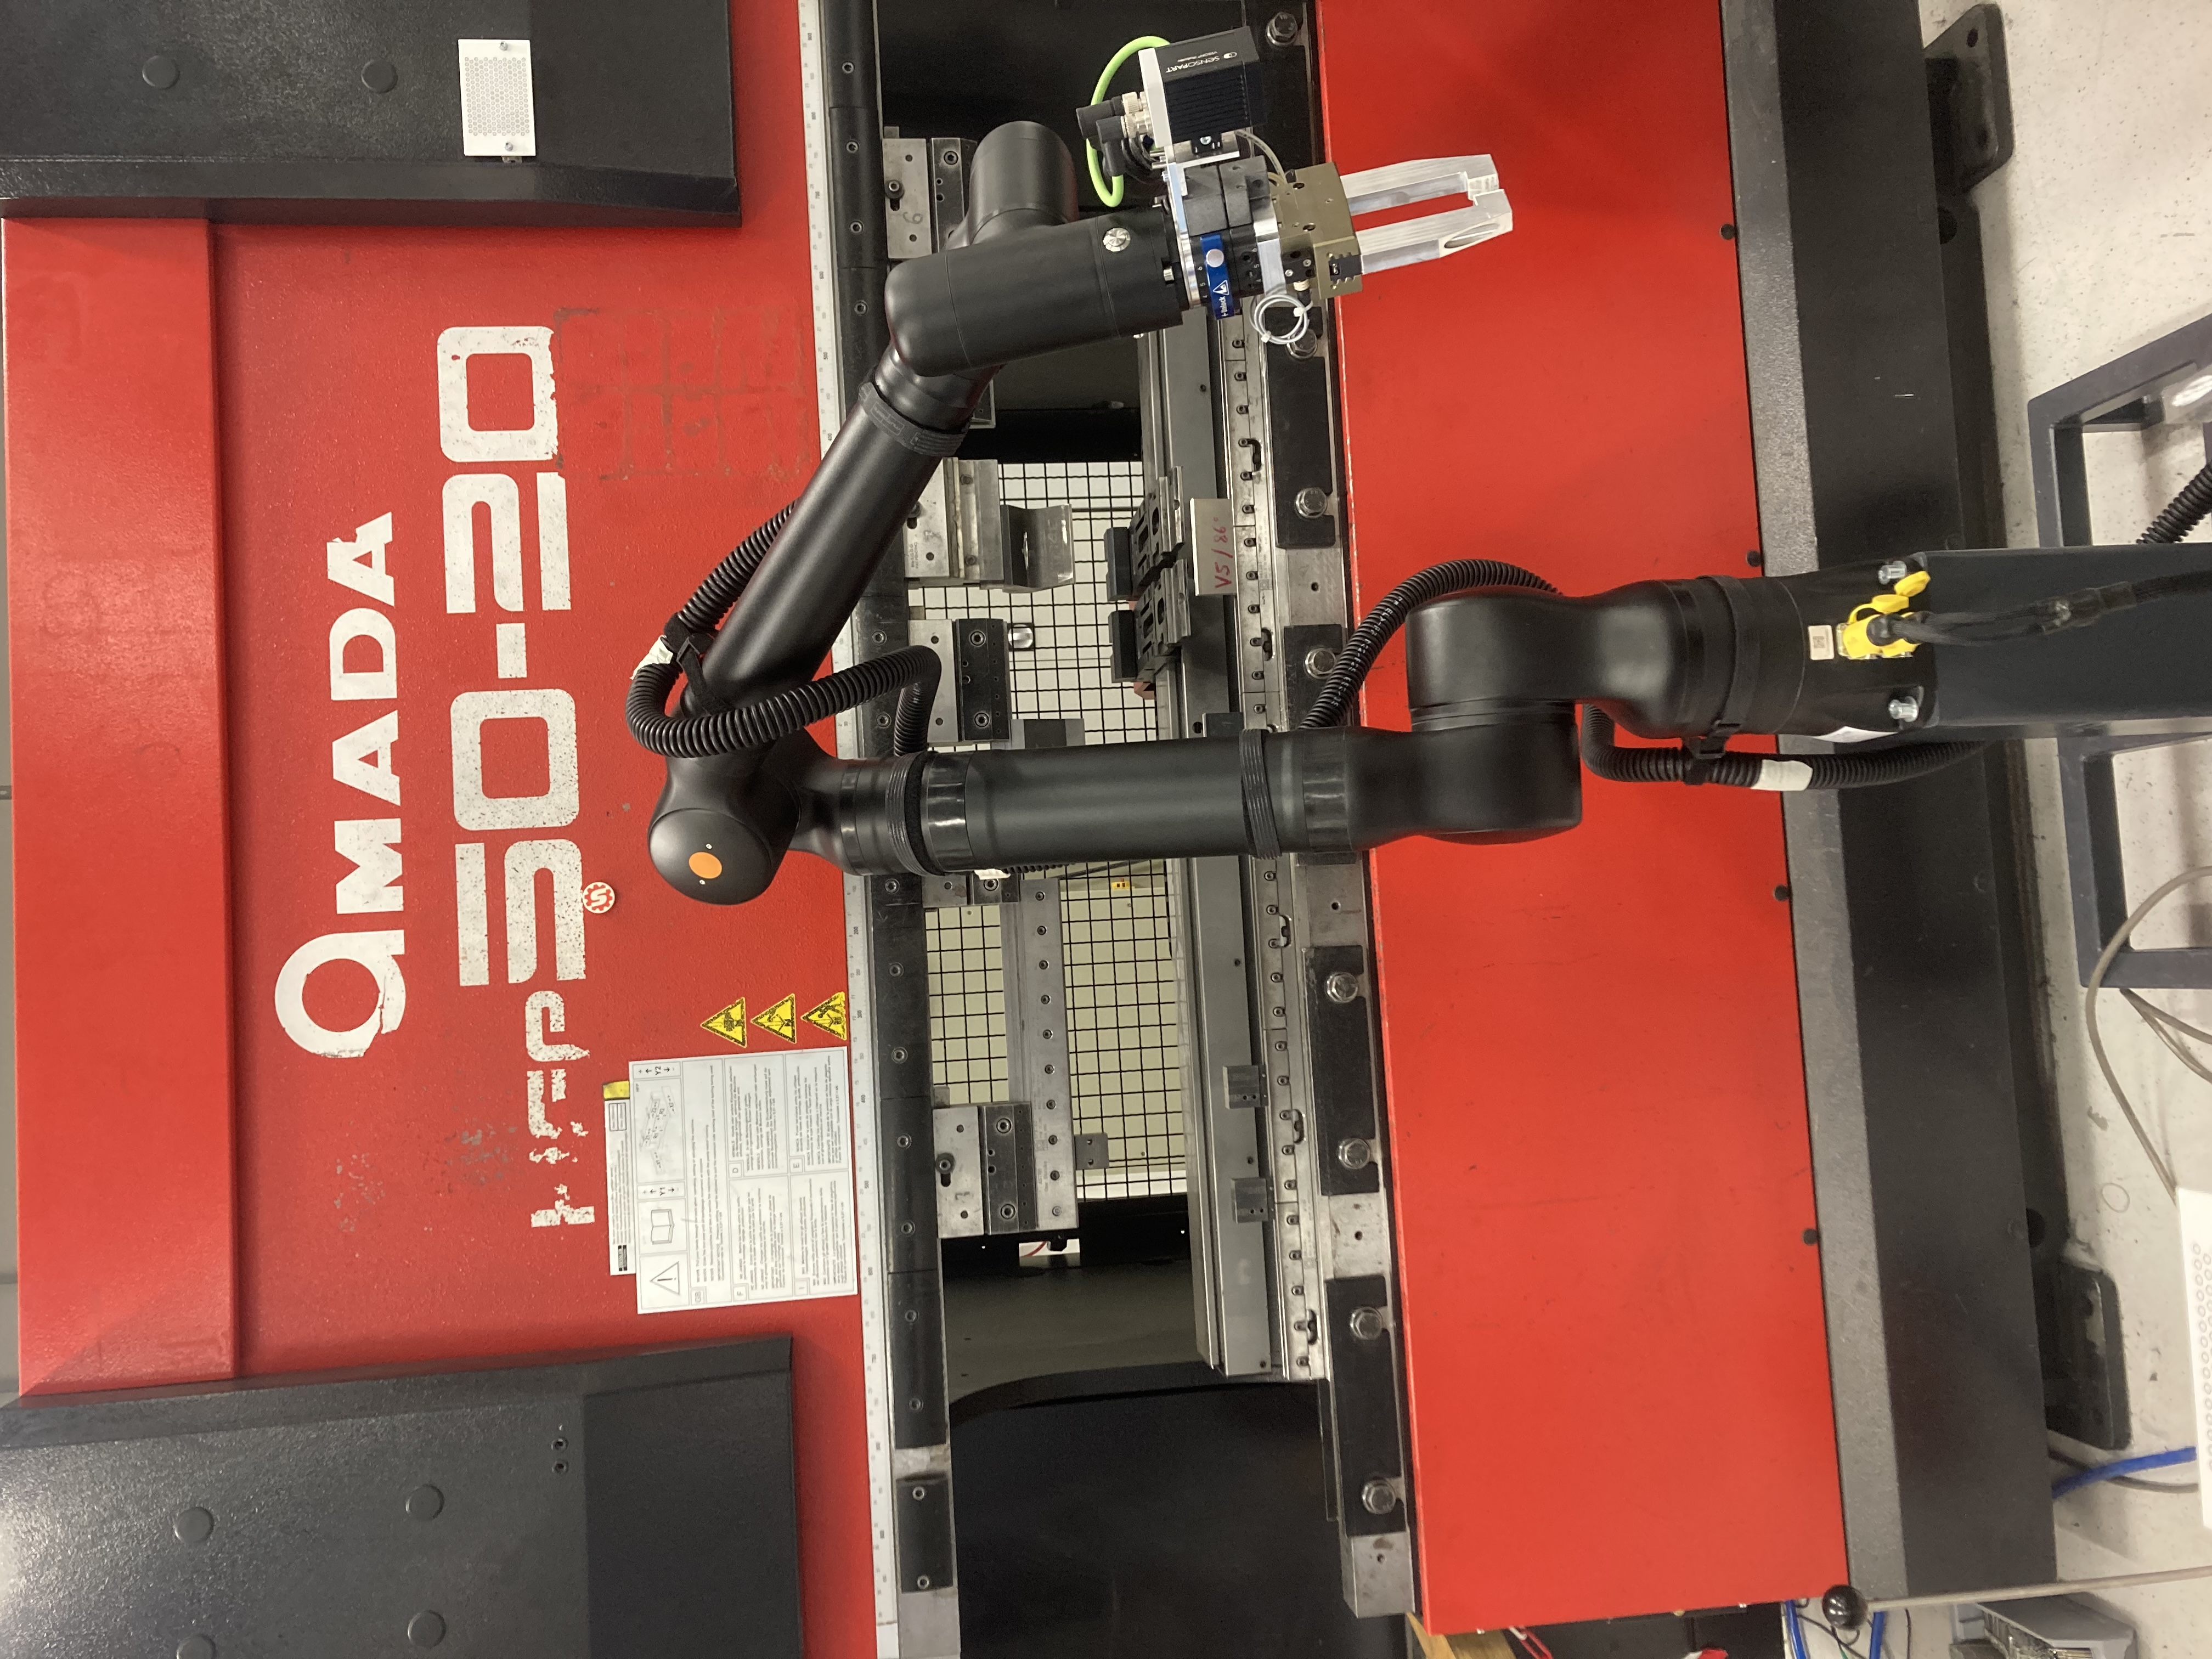
\includegraphics[width=1\textwidth]{figures/handling-robot.png}
    \caption{Three bending stations for the bending operation}
    \caption{Components of the robot unit: 1) robot base 2) KR1410 manipulator 3) manual quick-change system 4) robotic gripper 5) robotic camera}
    \label{fig:robot-installation}
\end{figure}



\subsubsection{Robot base}
The base is a simply welded construction made of steel. The choice of steel material ensures that the base has
sufficient dead weight so that it can be transported together with the robot and gripper using a pallet
truck without the risk of tipping over. During operation, the robot unit is fixed to the floor with four M12
screws. 

\subsubsection{KR1410 manipulator}
The robot used is a 7-axis robot from Kassow Robots with model KR1410. This robot model fulfills the requirements defined in 
the section \ref{sec:requirements}. Simulations have shown that this robot is above to reach even the lowest drawers of the shelf of the
storage station. Two full rotations (720\textdegree) of five out of seven joints allows complex motions in limited space.
A flexible conduit containing pneumatic hose for the pneumatic parallel gripper and communication cable for the camera goes around the manipulator to reach the end-effector.



\subsubsection{Manual quick-change system}
The gripper is attached to a manual quick-change
system. The manual quick-change system makes it possible to exchange different gripper
designs in a short time and without increased effort if required for a sheet metal part type. Sheet metal
part is folded into something like a box. The quick-change system also has an electric and pneumatic power feed-through, which ensures simple,
user-friendly changeover.

\subsubsection{Robotic Gripper}
The gripper is a Schunk pneumatic parallel gripper. It is powered and controlled by the Tool-IO board on the KR1410.
The robotic gripper grips an object with an applied pressure of five bar. This is enough to hold the sheet metal part
in place during motion of the arm. 
The fingers are made from aluminum material and fingertips are \hyperref[acro:3D]{3D} printed using a \hyperref[acro:FDM]{FDM} printer.  The tips are worn out
after some period of time, but are easily replaceable by \hyperref[acro:3D]{3D} printing.
In the program tree, the center of fingertips sets the \hyperref[acro:TCP]{TCP} for the robot and is 216 mm from the \hyperref[acro:TFC]{TFC}.


\subsubsection{Robotic Camera}
A camera system is installed on the robot itself. This is used to determine the relative
position between the robot unit and the unloading station, bending machine and storage station using the markers
and between the robot unit and the sheet metal part (when it is first made available at the
unloading station or is gripped) using features on the sheet metal part.
As the working distance of this camera is large (300 mm), using external light source is required to protect against ambient light. 
This is because light reflections or changing extraneous light can distort evaluation results.
